\documentclass[../main.tex]{subfiles}

\begin{document}

Diferentes organizaciones, entre las que se incluye The American Journal of Psychiatry, han
presentado como una problemática creciente la sustitución de las interacciones sociales por las
interacciones a través de medios digitales (redes sociales), lo que de acuerdo con los expertos está correlacionado con problemas psicológicos (estrés, ansiedad, adicción). Con el propósito de realizar un estudio formal en cierta universidad, se propuso como primera etapa determinar si el tiempo, en minutos, que un estudiante dedica a visitar las redes sociales se puede modelar como una variable aleatoria con una distribución de probabilidad conocida, particularmente, si se asemeja a una distribución normal. Para el desarrollo de esta primera etapa, se hizo seguimiento al tiempo que una muestra aleatoria de 150 estudiantes dedica en las redes sociales diariamente. Los resultados de este seguimiento se presentan en el archivo de excel \textit{DatosRedesSociales.xlsx} .

\begin{enumerate}[(a)]

\item \textbf{(2 puntos)} Plantee la prueba de hipótesis nula y alterna de la prueba.
\begin{align*}
	H_0 : \text{Tiempo en redes} &= \mathcal{N}(121.22, 20.033^2) & H_1 : \neg H_0
\end{align*}

\item \textbf{(12 puntos)} Identifique el estadístico de prueba con su distribución y calcúlelo. Utilice 10 clases equiprobables.
$$\textbf{EP} \sim \mathcal{X}_{(10, 1)}^2 = \sum_{i = 1}^{10} \frac{\hat{o}_i - \hat{e}_i}{\hat{e}_i}$$
$\hat{o}$ es el valor observado y $\hat{e}$ es e valor esperado.

A continuación se muestran los intervalos y el estadístico de prueba.

\begin{figure}[h]
\centering
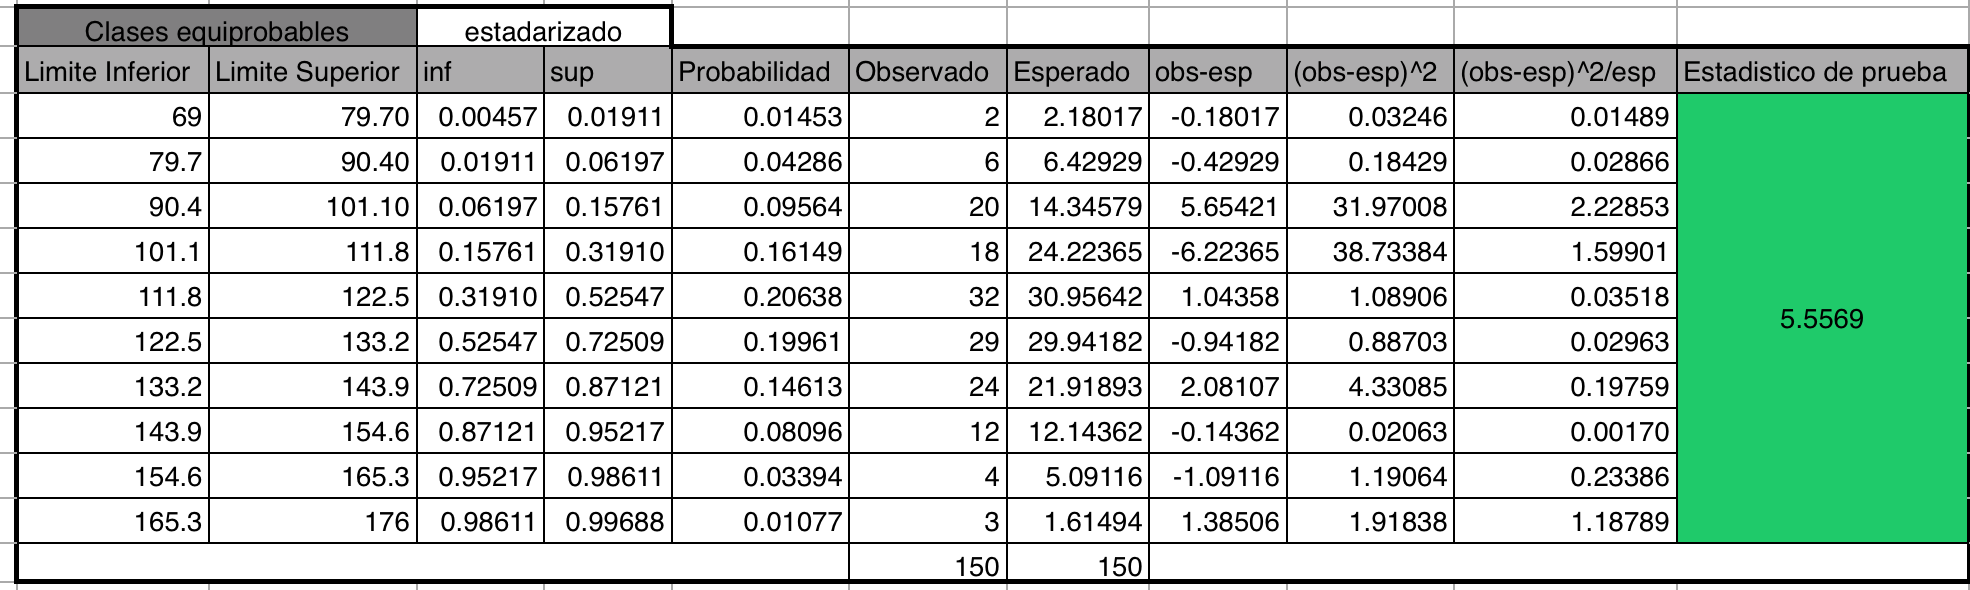
\includegraphics[width=13cm]{hipo.png}
\label{fig:img1}
\end{figure}

\pagebreak

\item \textbf{(4 puntos)} Utilizando un nivel de significancia del 5\%, realice una gráfica de la distribución del estadístico de prueba, identifique el punto crítico y la región de rechazo.
Adicionalmente, ubique el valor del estadístico de prueba.

\begin{figure}[h]
\centering
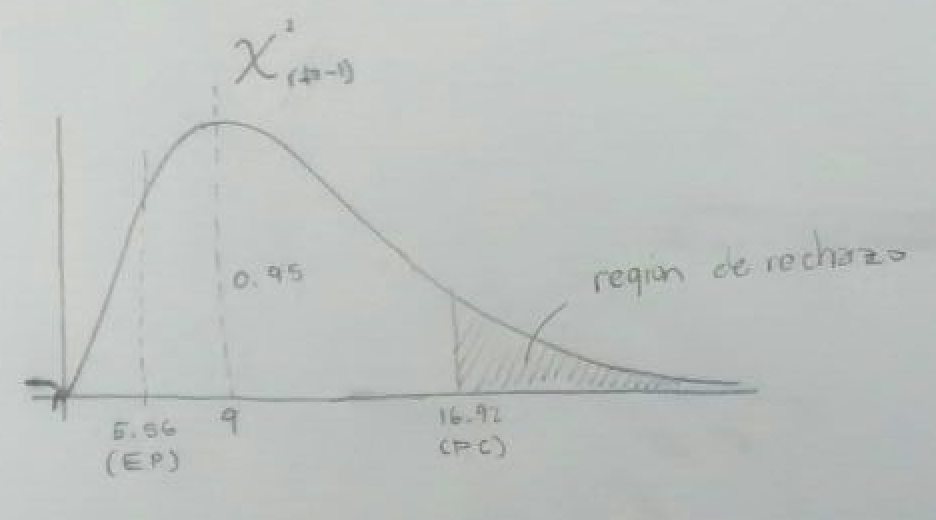
\includegraphics[width=13cm]{ugg.png}
\label{fig:img1}
\end{figure}

\item \textbf{(2 puntos)} Concluya en términos del problema.

Al comparar el estadístico de prueba con la región crítica, se observa que el estadístico de prueba, es menor al punto crítico, por lo que no está en la región de rechazo. Entonces, existe evidencia estadística para no rechazar la hipótesis nula, y de hecho, se puede afirmar que la muestra se distribuye normal.

\end{enumerate}

\end{document}
